\documentclass[journal]{IEEEtran}
\usepackage[spanish,english]{babel}
\usepackage[T1]{fontenc}
\usepackage{cite}
\usepackage{array}
\usepackage{url}
\usepackage{amsmath}
\usepackage{tikz}
%\usepackage{subfig}
\usepackage{amsfonts}
\usepackage{float}
\usepackage{amssymb}
\usepackage{enumerate}
\usepackage{hyperref}
\usepackage{pstricks}
\usepackage{pictex}
\usepackage{pst-all}
\usepackage{multicol}
\usepackage{booktabs}
\usepackage{siunitx} 
\hyphenation{neo-or-to-do-xia bio-ae-ro-sol}

\begin{document}

\title{Control de motor por PWM definido por entradas de teclado}
\author{Rafael Ricardo Galindo León, Santiago Andrés García Benitez\\
        (rrgalindol, saagarciabe)@unal.edu.co}

\markboth{Control de motor por PWM definido por entradas de teclado}
{Shell \MakeLowercase{\textit{et al.}}: Bare Demo of IEEEtran.cls for IEEE Journals}

\maketitle
\begin{otherlanguage}{english} 
\begin{abstract}
This report corresponds to the development of a PWM motor control defined by keyboard inputs, using microcontrollers. The circuit was depeloped with 1 DC motor and 1 L9110S H-Bridge as the motor driver.
\end{abstract}
\begin{IEEEkeywords}
Arduino, Interrupts, PWM, Serial Communication.
\end{IEEEkeywords}
\end{otherlanguage}
\IEEEpeerreviewmaketitle
\begin{otherlanguage}{spanish}
\section{Introducción}
\IEEEPARstart{C}{o}mo último concepto que se puede incluir en el manejo básico de los Microcontroladores se encuentra en de generación PWM. La Modulación de Ancho de Pulso (PWM, por sus siglas en inglés), es una técnica de ingeniería altamente difundida por su facilidad de implementación y sus numerosas ventajas. Particularmente, en el área de control de motores es ampliamente utilizado. Lo anterior, debido a que, mediante la modificación del ciclo útil de una señal cuadrada, permite generar distintos niveles de RMS partiendo de una tensión de alimentación fija. En una aplicación como el Control de motor por PWM definido por entradas de teclado se hace uso directo de esta funcionalidad en un microcontrolador.  

\section{Desarrollo}

\subsection{Montaje}
Como primer acercamiento al desarrollo de la práctica, inicialmente se planteó el Diagrama de conexiones del Contador. Para esto se hizo uso del software KiCad, en el que se realizaron las conexiones respectivas para el Puente H y el motor. A su vez, se planteó la conexión para la comunicación serial teniendo en cuenta el Data Sheet del Microcontrolador. De esta manera en la Figura \ref{E} se puede observar el planteamiento de la propuesta para el circuito a desarrollar. Teniendo esta primera fase definida, se procedió a realizar el Montaje en Protoboard del Control de motor.

\begin{figure}[H]
    \centering
    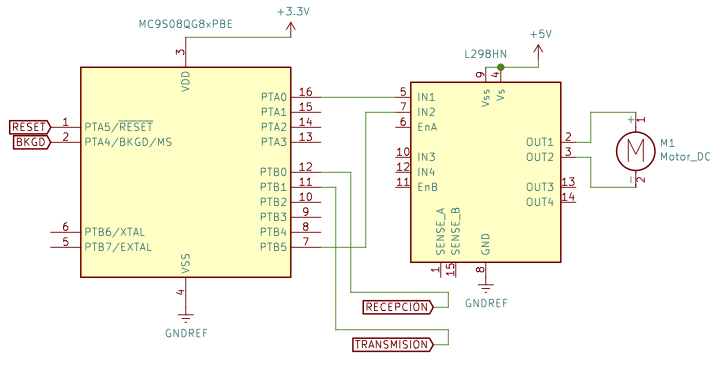
\includegraphics[scale=0.32]{Imágenes/Esquema6.jpg}
    \caption{Esquemático}
    \label{E}
\end{figure}

Para la construcción del Control de motor se utilizó el Microcontrolador MC9S08QG8 de la familia HCS08 de Motorola Freescale. A este se conectó un Puente H L298N. Al Puente H se conectó un motor DC. El montaje se puede observar en la Figura \ref{M}.

\begin{figure}[H]
    \centering
    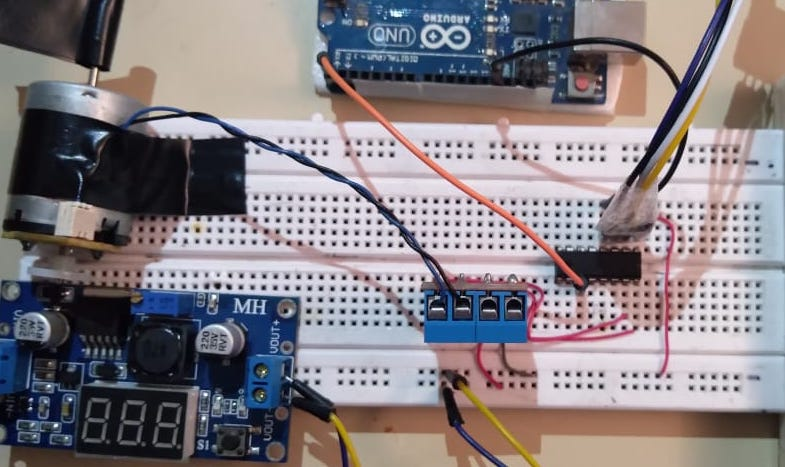
\includegraphics[scale=0.28]{Imágenes/Montaje_Practica_6.jpeg}
    \caption{Montaje en Protoboard}
    \label{M}
\end{figure}

Para la sección del montaje correspondiente al las salidas del Microcontrolador al Puente H se designaron los pines PTA0 y PTA1 del QG8. Dichos puertos del MCU se conectaron al Puente-H L298N a través de los pines In1 e In2, respectivamente. A su vez, se conectaron las dos terminales del motor a los pines Out1 y Out2 del Puente-H L298N.\\

También se designaron los pines PTB0 y PTB1 para la comunicación serial ya que estos corresponde al Rx y Tx del periférico de comunicación serial diseñado para cumplir la labor de recepción y transmisión de datos, respectivamente.

\subsection{Programación}

Para el desarrollo de la lógica del Control de motor se utilizó el programa CodeWarrior 10.7. El código se escribió en C.\\

El algoritmo del funcionamiento del Control de motor se planteó de la siguiente manera. Se definieron las tareas de: leer la entrada de teclado, asignar el valor de PWM y transmitir el valor de PWM. A continuación, en la Figura \ref{DDF_General} se presenta el Diagrama de Flujo correspondiente al Control de motor.

\begin{figure}[H]
    \centering
    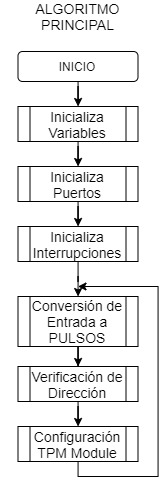
\includegraphics[scale=.6]{Imágenes/Practica 6.2.jpg}
    \caption{Diagrama de Flujo General del algoritmo}
    \label{DDF_General}
\end{figure}

Con respecto a la lectura de las entradas de teclado, se hace uso del canal de recepción serial Rx. Cuando se recibe información por este canal, se guarda dicha información para luego compararla con una tabla de correspondencia que se tiene establecida por las condiciones de la aplicación. En esta, cada tecla del computador corresponde a un porcentaje de PWM (11 teclas) o a un signo de giro (2 teclas). En la Figura \ref{DDF_Serial} se muestra la rutina de lectura del canal Rx.

\begin{figure}[H]
    \centering
    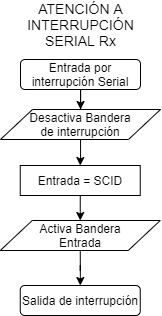
\includegraphics[scale=.6]{Imágenes/Practica 6.1.jpg}
    \caption{Diagrama de Flujo Interrupción Serial Rx}
    \label{DDF_Serial}
\end{figure}

Para la asignación del valor del PWM simplemente se toma, de la tabla de correspondencias generada, el valor necesario para el registro del PWM. Luego, se procede a asignarle el número correspondiente al registro de Valor del Canal. A continuación se presenta dicha tabla de correspondencias:

\begin{table}[H]
        \label{Salidas}
        \centering
        \caption{Código de velocidades}
        \begin{tabular}{||c||c||c||}
        \hline \hline 
        {\centering \textbf{Tecla}} & {\centering \textbf{\% Ciclo Útil}} & {\centering \textbf{TPMCnV}} \tabularnewline \hline
        0 & 0 & 0 \tabularnewline \hline
         1 & 10 & 400 \tabularnewline \hline
         2 & 20 & 800 \tabularnewline \hline
         3 & 30 & 1200 \tabularnewline \hline
         4 & 40 & 1600 \tabularnewline \hline
         5 & 50 & 2000 \tabularnewline \hline
         6 & 60 & 2400 \tabularnewline \hline
         7 & 70 & 2800 \tabularnewline \hline
         8 & 80 & 3200\tabularnewline \hline
         9 & 90 & 3600\tabularnewline \hline
         T & 100 & 4000\tabularnewline \hline
         \hline
         P & + &  \tabularnewline \hline
         N & - &  \tabularnewline \hline
        \hline 
        \end{tabular}
    \end{table}

Finalmente, en la transmisión del valor de PWM, se hace uso del canal de transmisión serial Tx para presentar el valor del \% de Ciclo Útil del PWM en el monitor.

\subsection{Comprobación}
En el desarrollo de esta aplicación hubo algunos detalles a tener en cuenta o revisar para asegurar un adecuado funcionamiento. El primero, como se ha venido haciendo mención en prácticas anteriores, tiene que ver con la comunicación serial. Es necesario hacer una sincronización entre el Baud Rate del microcontrolador y el del monitor. Esto con el fin de que pueda existir comunicación entre los dos sin que se pierda información o se esté operando a una velocidad diferente. Además, es necesario implementar los retardos necesarios para la lectura y la transmisión. Al entender la forma en la que está implementada la comunicación serial, se observa la necesidad de esperar a que la información se envíe o se reciba en su totalidad.\\

Con respecto a la configuración del módulo de PWM del microcontrolador, al observar la fórmula que lo determina, es posible detectar que solo uno de los factores tiene la posibilidad de modificarse por código. Ya que la Frecuencia de Bus es fija en el microcontrolador, la escogencia del módulo (y su cálculo) dependería exclusivamente de la frecuencia de PWM que se quiera trabajar. Por ejemplo para trabajar con una frecuencia de 1kHz se obtendría un módulo de 3999 (que es el que se ha seleccionado para esta aplicación).\\

Sin embargo, cabe mencionar que sería posible modificar la Frecuencia de Bus haciendo uso de una estrategia física. Al conectar un reloj externo (cristal, oscilador), sería posible, habilitando la entrada de un Oscilador Externo al microcontrolador, modificar también la Frecuencia de Bus. De esta manera, se tendría un rango más amplio de frecuencia de PWM para escoger a través del módulo de PWM.\\

Es posible observar que la implementación del PWM, habiendo establecido el módulo (definiendo la frecuencia), es relativamente simple. Basta con cambiar el valor que se carga al Registro del Canal de manera que tenga correspondencia con el valor de PWM que se espera. Esto se puede corroborar al examinar la Tabla 1 en la que se observa que los valores cargados a TPMCnV corresponden al porcentaje mencionado en la tabla del valor del módulo de PWM (por ejemplo, 800 es el 20\% de 4000, 2800 es el 70\% de 4000, entre otros).\\

Por la misma línea, también es posible observar que el cambio de signo del PWM es igualmente sencillo. Solo basta invertir los valores que se cargan en los Registros de Status y Control. Si para un signo uno de los canales (0) se carga con cero y el otro (1) con un valor diferente de cero; para invertir el signo, se carga el canal (0) que estaba cargado con cero con un valor diferente de cero y el otro (1) con cero.\\

Por último, es valioso mencionar que en esta práctica, igual que en la anterior, fue posible descubrir y aprovechar las ventajas que presenta el lenguaje C sobre el lenguaje Assembly en algunas aplicaciones.

\section{Conclusiones}
\begin{enumerate}
    \item Las Señales PWM son muy usadas en los controles que requieren variar la tensión RMS para hacer algún tipo de control. Sin embargo es importante entender que este método tiene ciertas limitaciones como por ejemplo el ruido que puede generar una señal cuadrada de alta frecuencia y el impacto que esto puede tener en los dispositivos que se controla.
    \item En sistemas de motores eléctricos controlados por señales PWM se debe hacer un cálculo para determinar la frecuencia mínima a la que el motor responde a la señal PWM como una señal análoga.
    \item Es bueno recordar que la interfaz serial puede funcionar con solo un canal, en el cual se tenga solo envío o solo recepción de datos sin que esto afecte el funcionamiento. Esta característica es útil en los casos en que los canales de comunicación o los pines del microcontrolador son limitados.
    \item Ya que para que el motor opere se requiere de unos niveles de potencia y tensión que un microcontrolador no puede proveer, se requiere de una fuente de alimentación independiente y un driver que puedan recibir la señal de control aportada por el Microcontrolador y potenciarla para que se realice el proceso que se requiere sobre el motor.
\end{enumerate}

\begin{thebibliography}{1ente,5}
    \bibitem{NXP} NXP
    \textit{MC9S08QG8 - MC9S08QG4 Data Sheet.}
    Disponible en: https://www.nxp.com/docs/en/data- sheet/MC9S08QG8.pdf
 
\end{thebibliography}
\end{otherlanguage}
\end{document}